\documentclass[a4paper,11pt,fleqn]{article}%fleqn pour aligner les equations à gauche
\usepackage{../../Styles/Exercice}


\newcommand{\chnum}{Chapitre 06}
\newcommand{\chtitle}{Quantité de matière}
\newcommand{\dtype}{TP}

\begin{document}
\maketitle

\section{Nombre de molécules et de moles}
	\subsection*{Document 1 : Masse des atomes}
	\begin{tabular}{|>{\arraybackslash}m{2.5cm}|>{\arraybackslash}m{3.5cm}|>{\arraybackslash}m{3.5cm}|>{\arraybackslash}m{3.5cm}|>{\arraybackslash}m{3.5cm}|}
	\hline
	Atome & Hydrogène & Carbone & Oxygène & Potassium \\
	\hline
	Masse (kg) & $m_H = 1,67 \times 10^{-27}$ & $m_C = 1,99 \times 10^{-26}$ & $m_0 = 1,66 \times 10^{-26}$ & $m_K = 6,49 \times 10^{-26}$\\
	\hline
	\end{tabular}
	\subsection*{Document 2 : Le saccharose, constituant principale du sucre de table}
	\begin{tabular}{>{\centering \arraybackslash}m{6cm}>{\centering \arraybackslash}m{6cm}>{\centering \arraybackslash}m{6cm}}
	Modèle moléculaire du saccharose : & Formule brute : & Morceaux de sucre : \\
	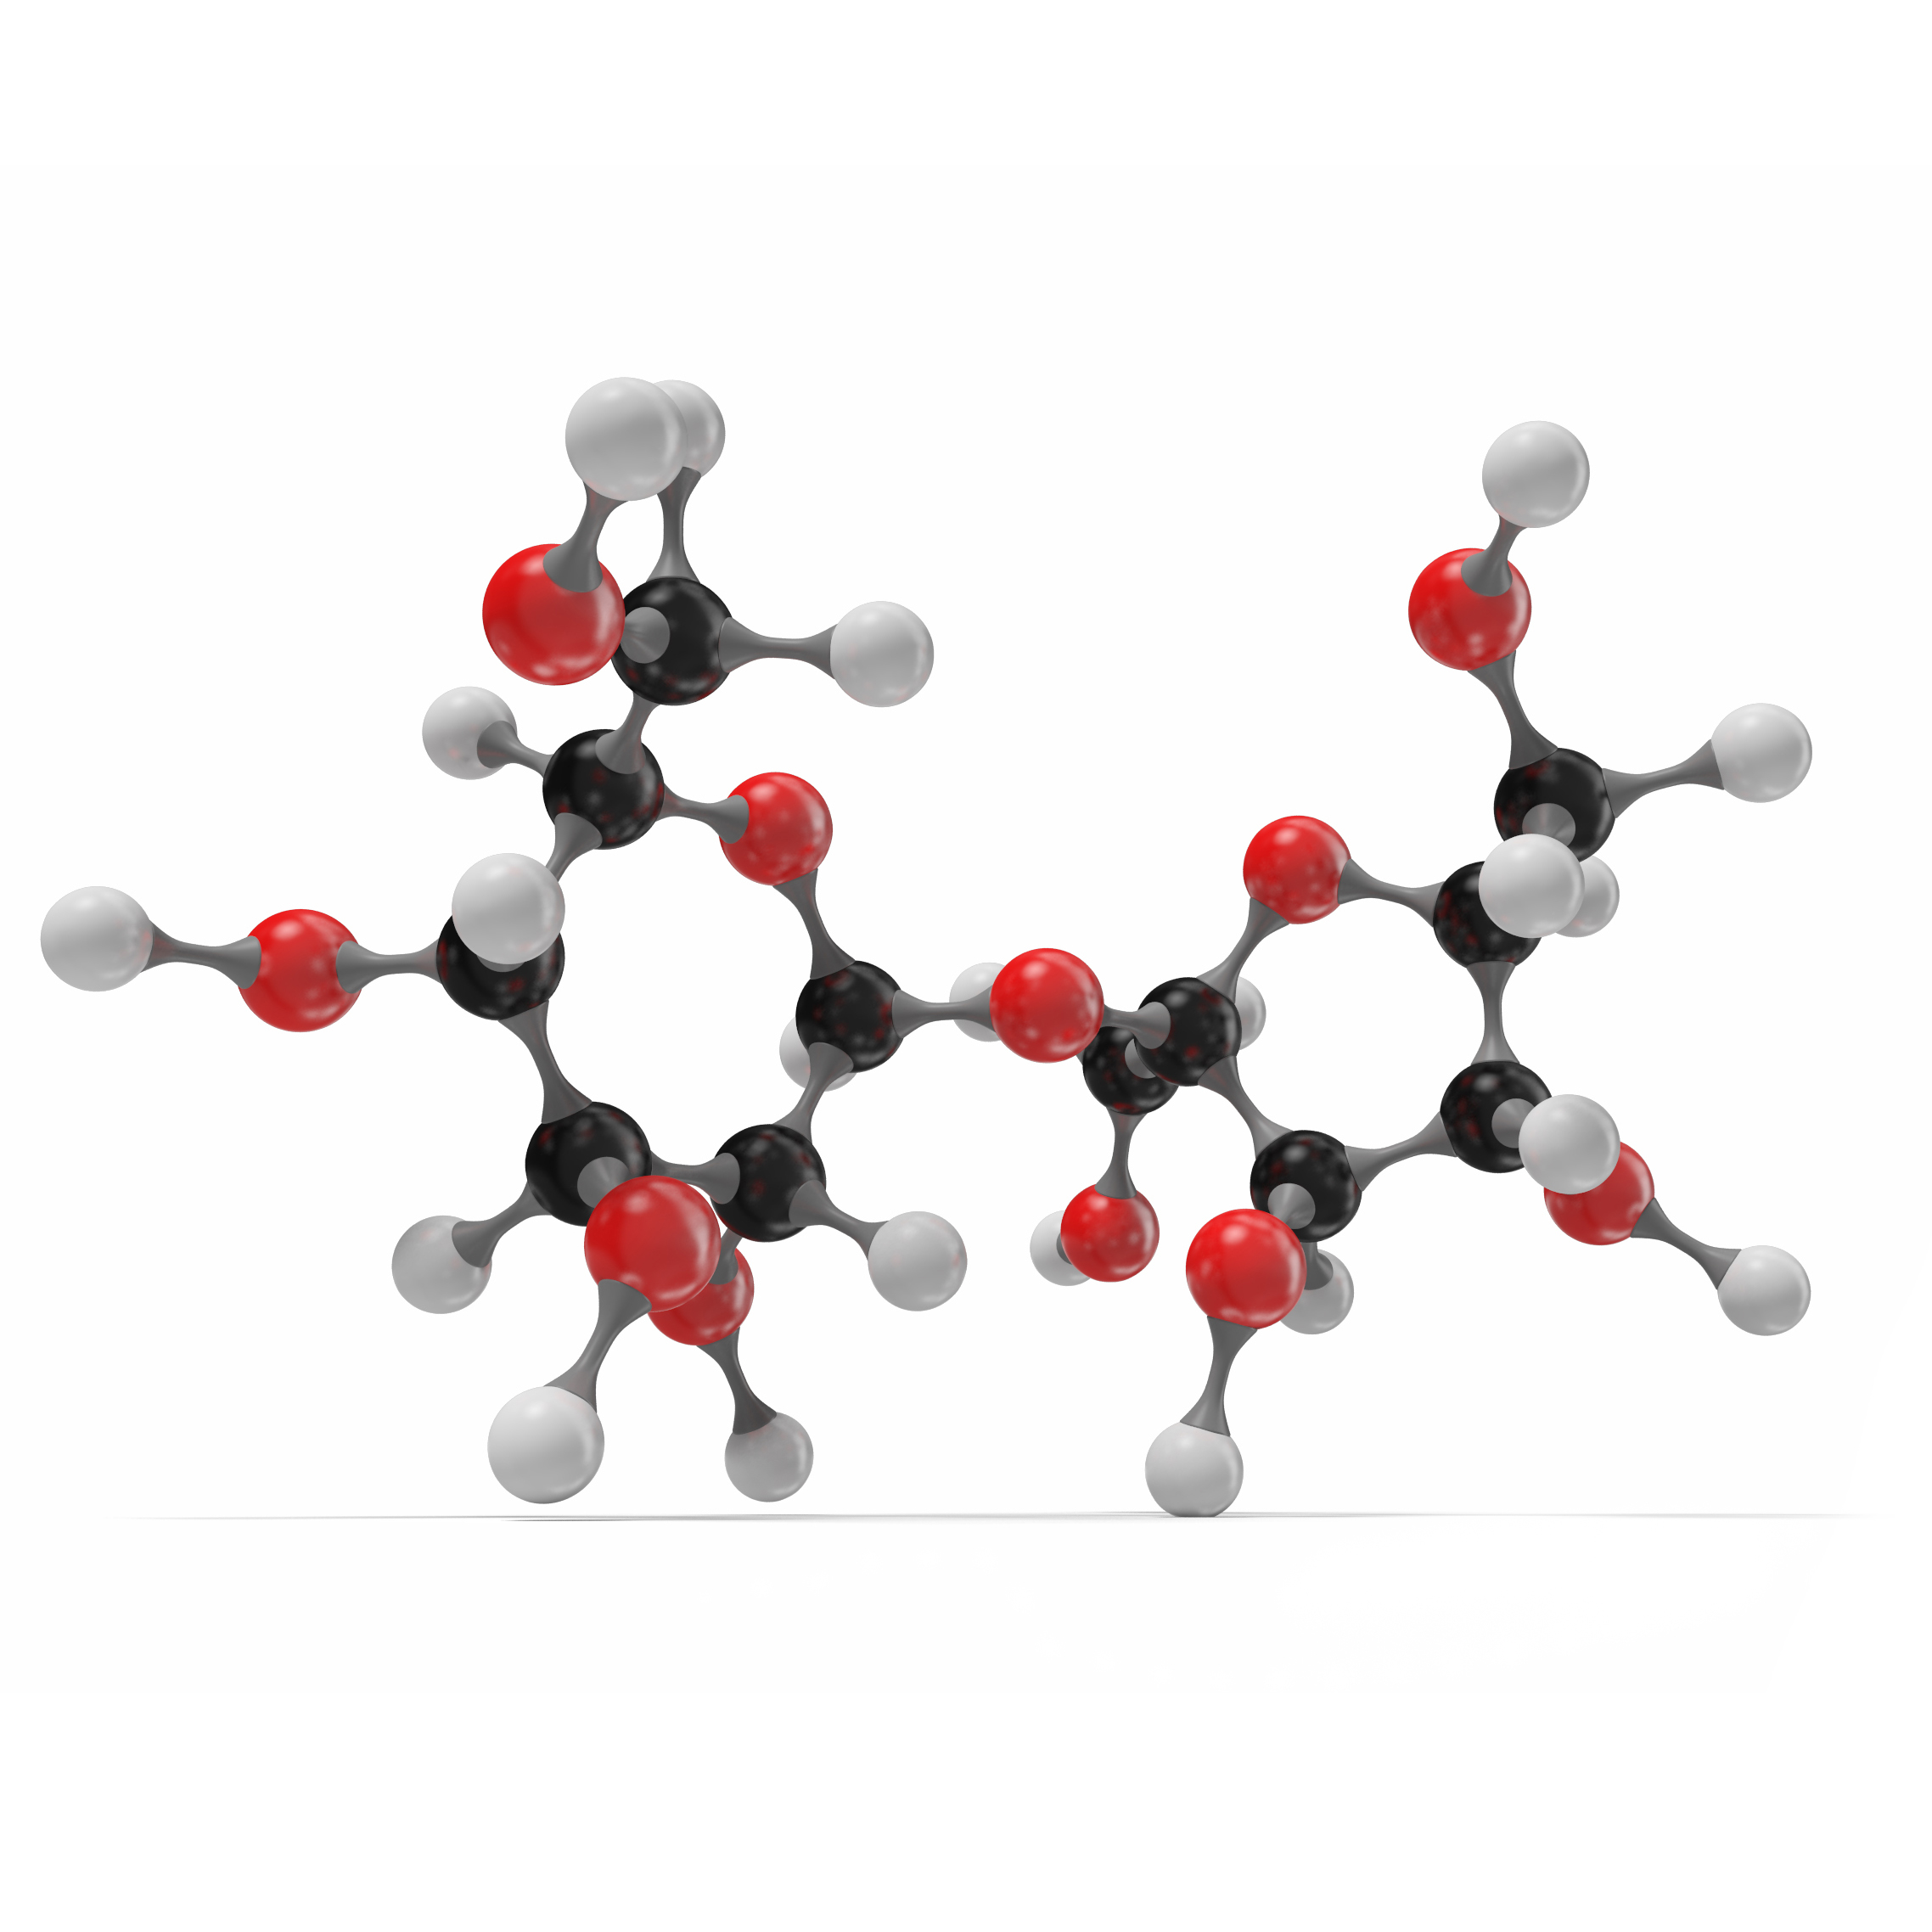
\includegraphics[scale=.04]{Ressources/Saccharose3D.jpg}&$C_{12}H_{22}O_{11}$ &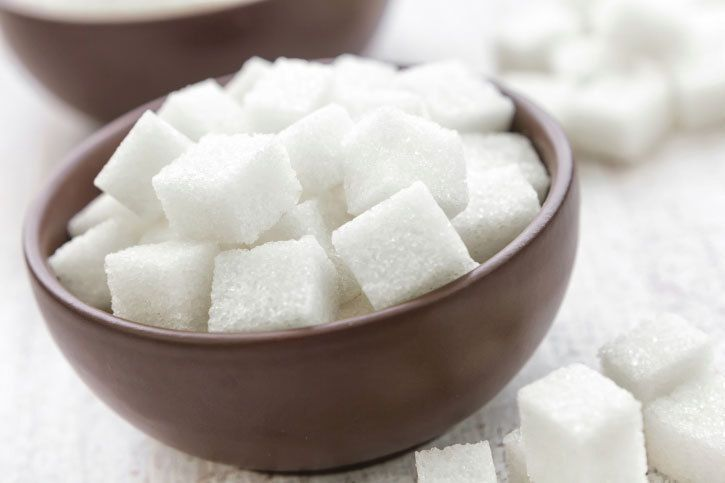
\includegraphics[scale=.1]{Ressources/Sucres.jpg}\\
	\end{tabular}
	\subsection*{Document 3 : La mole}
	Pour compter les très nombreuses entités présentes dans un échantillon, les chimistes les regroupent par paquets appelés moles. Une mole contient $N_A = 6,022 \times 10^{23}$ entités chimiques (molécules, atomes, ions).
	\subsection*{Questions : }
	\begin{enumerate}
		\item Calculer la masse $m_{Sac}$ d'une molécule de saccharose en détaillant la démarche.\\
		\begin{tikzpicture}
		\draw (0, 0) -- (18, 0) -- (18, 5) -- (0, 5) -- (0, 0);
		\end{tikzpicture}
		\item Grâce à une balance électronique, déterminer le nombre $N$ de molécules de saccharose contenues dans un morceau de sucre.\\
		\begin{tikzpicture}
		\draw (0, 0) -- (18, 0) -- (18, 5) -- (0, 5) -- (0, 0);
		\end{tikzpicture}
		\item Combien de moles $n$ de saccharose contient une spatule de sucre ?\\
		\begin{tikzpicture}
		\draw (0, 0) -- (18, 0) -- (18, 5) -- (0, 5) -- (0, 0);
		\end{tikzpicture}
	\end{enumerate}
\section{Le liquide magique}
	\subsection*{Protocole :}
Un protocole détaillant l'élaboration d'un liquide magique a été trouvé :
\begin{enumerate}
	\item Dans un erlenmeyer de 250 mL, introduire $4,2 \times 10^{24}$ molécules d'eau.
	\item Prélever à l'aide d'une spatule, $9,6 \times 10^{21}$ molécules de saccharose en poudre et les introduire dans l'erlenmeyer.
	\item Ajouter (SANS LES TOUCHER) $0,06$ mol d'hydroxyde de potassium KOH.
	\item Verser 3 gouttes de bleu de méthylène, boucher agiter et laisser reposer.
\end{enumerate}
	\subsection*{Réalisation :}
Votre mission : à l'aide des informations précédentes des documents 1 et 3, réécrire le protocole en précisant les masses des différentes espèces chimiques à prélever pour réaliser le liquide magique. Après validation par le professeur, réaliser ce protocole en respectant les règles de sécurité.\\
\begin{tikzpicture}
\draw (0, 0) -- (19, 0) -- (19, 11) -- (0, 11) -- (0, 0);
\end{tikzpicture}
\end{document}